%%%%%%%%%%%%%%%%%%%%%%%%%%%%%%%%%%%%%%%%%%%%%%%%%%%%%%%%%%%%%%%%%%%%%%%%

%%% LaTeX Template for AAMAS-2021 (based on sample-sigconf.tex)
%%% Prepared by Natasha Alechina and Ulle Endriss (version 2020-08-06)

%%%%%%%%%%%%%%%%%%%%%%%%%%%%%%%%%%%%%%%%%%%%%%%%%%%%%%%%%%%%%%%%%%%%%%%%

%%% Start your document with the \documentclass command.
%%% Use the first variant below for the final paper.
%%% Use the second variant below for submission.

\documentclass[sigconf]{aamas} 
%\documentclass[sigconf,anonymous]{aamas} 

%%% Load required packages here (note that many are included already).

%%%%%%%%%%%%%%%%%%%%%%%%%%%   MACROS   %%%%%%%%%%%%%%%%%%%%%%%%%%%%%%%%%

\newcommand{\xmu}[2]{x_{#1_#2}^{#2}(t)}
\newcommand{\xmudash}[2]{x_{#1_#2}^{#2}(t')}
\newcommand{\payoff}[2]{P^{#2}_{#1_#2, #1_{-#2}}}

\newcommand{\dxmu}[1]{\dot{x}_{#1_\mu}^{\mu} (t)}
\newcommand{\hxmu}[1]{\hat{x}_{#1_\mu}^{\mu} (t)}
\newcommand{\hxnu}[1]{\hat{x}_{#1_\nu}^{\nu} (t)}
\newcommand{\hxmudash}[1]{\hat{x}_{#1_\mu}^{\mu} (t')}
\newcommand{\hxnudash}[1]{\hat{x}_{#1_\nu}^{\nu} (t')}

\newcommand{\txmu}[2]{\tilde{x}_{#1_#2}^{#2}(t)}
\newcommand{\dtxmu}[2]{\dot{\tilde{x}}_{#1_#2}^{#2}(t)}
\newcommand{\tpayoff}[2]{\tilde{P}^{#2}_{#1_#2, #1_{-#2}}}
\newcommand{\talpha}{\tilde{\alpha}}
\newcommand{\ttau}{\tilde{\tau}}
\newcommand{\htau}{\hat{\tau}}
\newcommand{\xfixed}{x_\infty}
\newcommand{\ezerof}{\eta_{0, \infty}}
\newcommand{\eonef}{\eta_{1, \infty}}

\newcommand{\xpert}{\hat{x}(t)}
\newcommand{\xpertdash}{\hat{x}(t')}
\newcommand{\ezeropert}{\hat{\eta}_0(t)}
\newcommand{\eonepert}{\hat{\eta}_1(t)}

\newcommand{\eom}{\frac{\dxmu{i}}{\xmu{i}{\mu}} - \alpha \ttau \left ( \sum_{i_{-\mu}} \payoff{i}{\mu} \prod_{\kappa \neq \mu} \xmu{i}{\kappa} \right ) + \\ \alpha \htau \left ( \frac{1}{\sqrt{N}} \sum_{i_\mu i_{-\mu}} \xmu{i}{\mu} \payoff{i}{\mu} \prod_{\kappa \neq \mu} \xmu{i}{\kappa} \right ) - \talpha \rho^{\mu}_{i}(t)}

%%%%%%%%%%%%%%%%%%%%%%%%%%%%%%%%%%%%%%%%%%%%%%%%%%%%%%%%%%%%%%%%%%%%%%%%

%%% AAMAS-2021 copyright block (do not change!)

\setcopyright{ifaamas}
\acmConference[AAMAS '21]{Proc.\@ of the 20th International Conference on Autonomous Agents and Multiagent Systems (AAMAS 2021)}{May 3--7, 2021}{London, UK}{U.~Endriss, A.~Now\'{e}, F.~Dignum, A.~Lomuscio (eds.)}
\copyrightyear{2021}
\acmYear{2021}
\acmDOI{}
\acmPrice{}
\acmISBN{}

%%%%%%%%%%%%%%%%%%%%%%%%%%%%%%%%%%%%%%%%%%%%%%%%%%%%%%%%%%%%%%%%%%%%%%%%

%%% Use this command to specify your EasyChair submission number.
%%% In anonymous mode, it will be printed on the first page.

\acmSubmissionID{???}

%%% Use this command to specify the title of your paper.

\title[InstabilityinMARL]{Instability in Multi Agent Reinforcement Learning}

%%% Provide names, affiliations, and email addresses for all authors.

\author{Aamal Hussain}
\affiliation{
  \department{Department of Computing}
  \institution{Imperial College London}}
\email{aamal.hussain15@imperial.ac.uk}

\author{Francesco Belardinelli}
\affiliation{
  \department{Department of Computing}
  \institution{Imperial College London}}
\email{francesco.belardinelli@imperial.ac.uk}


%%% Use this environment to specify a short abstract for your paper.

\begin{abstract}
Modelling the dynamics of Q-Learning is an active and important topic for the sake of developing an {\em a priori} understanding of Reinforcement Learning. In this paper, we use methods from evolutionary game theory to analyse the stability of Q-Learning in $p$-player games, where payoffs are randomly generated. We determine the parameter range in which Q-Learning is expected to settle to a stable fixed point and the range in which the dynamics are unstable. 

This study allows for parameters to be appropriately chosen to ensure the safe convergence of a learning algorithm and as a first step towards understanding the range of behaviours that can be displayed by learning using the Q-Learning algorithm. We validate our theoretical results through numerical simulation and show that, within the bounds of experimental error, the region of instability can be characterised by the learning dynamics. We also note a few important implications of the study: 1) convergence is rare in Multi-Agent Reinforcement Learning. It is found that convergence to a unique fixed point occurs for simple games with 2 players and 2 actions. However, once either of these increase, convergence no longer occurs. 2) the existence of instability is not affected by the structure of the game itself. In fact, at least in the competitive regime, the payoff structure does not affect whether the game converges or not. 3) Convergence is guaranteed for low step-lengths but rapidly decreases as the step length increases. 
\end{abstract}

%%% The code below was generated by the tool at http://dl.acm.org/ccs.cfm.
%%% Please replace this example with code appropriate for your own paper.


%%% Use this command to specify a few keywords describing your work.
%%% Keywords should be separated by commas.

\keywords{Auction Theory, Reinforcement Learning, Social Simulation}

%%%%%%%%%%%%%%%%%%%%%%%%%%%%%%%%%%%%%%%%%%%%%%%%%%%%%%%%%%%%%%%%%%%%%%%%

%%% Include any author-defined commands here.
         
\newcommand{\BibTeX}{\rm B\kern-.05em{\sc i\kern-.025em b}\kern-.08em\TeX}

%%%%%%%%%%%%%%%%%%%%%%%%%%%%%%%%%%%%%%%%%%%%%%%%%%%%%%%%%%%%%%%%%%%%%%%%

\begin{document}

%%% The following commands remove the headers in your paper. For final 
%%% papers, these will be inserted during the pagination process.

\pagestyle{fancy}
\fancyhead{}

%%% The next command prints the information defined in the preamble.

\maketitle 

%%%%%%%%%%%%%%%%%%%%%%%%%%%%%%%%%%%%%%%%%%%%%%%%%%%%%%%%%%%%%%%%%%%%%%%%

\section{Introduction}

Single agent reinforcement learning (RL) is a well established framework for allowing agents to learn optimal strategies when trained on an iterated task 
For a particularly strong example of this see \cite{Vinyals2019}. However, for the realisation of complex tasks, such as air traffic control, market negotiations and multi-robot coordination, it is required that the system be modelled as a multi-agent system (MAS). Such systems are not as well understood since a given agent is tasked with optimising a reward function which depends not only on a non-stationary environment, but also on the actions of other, possibly loosely coupled, agents \cite{SchwartzMulti-agentApproach}. 

It is, therefore, of paramount importance to develop a strong theoretical understanding of multi-agent reinforcement learning (MARL) to allow an {\em a-priori} understanding of the behaviour of a given learning algorithm. Fortunately, the study of MAS is not unique to the field of AI and has been extensively studied from the point of view of economics and game theory as well \cite{ShohamMultiagentFoundations}. In particular, the study of evolutionary game theory (EGT) considers the problem of a MAS which is repeatedly exposed to an iterated game. 
his idea shares a strong resemblance with MARL and, in fact, in \cite{Tuyls2006AnGames}, it was shown that, techniques from EGT may be fruitfully used to analyse Q-Learning \cite{Sutton2018}.

An important result in modelling such multi agent systems from the EGT perspective is that, when games are learnt and the assumptions of rationality and perfect information are lifted, games may not converge to an equilibrium. Instead, as shown in \cite{Sanders2018}, the dynamics may be more complex, and even chaotic (see Section~\ref{sec::DynamicalBehaviours}). The present work further describes that the emergence of such behaviours depends on the parameters of the games and the learning algorithm. For the analysis of multi-agent systems whose behaviour is inter-dependent, it is desirable that the system be such that the game convergence to a stable equilibrium. Without this, it is inherently impossible to predict the outcome of learning.  

\paragraph{Contribution}
In this study, we will be considering the question: under what choice of parameters is a
multi-agent system, which is trained on an iterated game using Q-Learning, likely to converge to an
equilibrium as opposed to displaying complex, or chaotic behaviours? In investigating this question, we will make the
following assumptions:

\begin{enumerate}
    \item There are a finite set of agent, though the size $p$ of the set is arbitrary. 
    \item The agents have a large, but discrete, strategy space: during the theoretical study, we
    will make the assumption that the number of actions $N$ goes to infinity.
    \item The agents are homogeneous. This requires that all agents have the same parameters and are
    trained using the same algorithm. Since this is typically the case in reinforcement learning
    studies, it is not an unreasonable assumption, but does present an interesting avenue for future
    work.
    \item The agents are trained on stateless, normal form games (i.e. the environment is static).
\end{enumerate}


\subsection{Related Work}

In this section we present an overview of the vast literature which considers the study of Reinforcement Learning (RL) from an evolutionary game dynamics perspective, as well as touching upon some important results and research within the field of game dynamics.

\paragraph{Evolutionary Game Dynamics} The theory of evolutionary game dynamics \cite{Morgenstern44} considers the case in which agents must repeatedly interact with one another. The outcome of this interaction depends on a payoff matrix; 'strong' strategies which maximise the reward are promoted whilst 'weaker' strategies diminish. The \textit{replicator dynamic} models this behaviour, and allows one to determine whether, after a number of iterations, the game is likely to converge to some fixed equilibrium and, if so, the probabilities with which strategies are played in this equilibrium. \cite{ShohamMultiagentFoundations} provides an excellent introduction to the replicator dynamic for the interested reader.

Analyses have been performed from the point of view of the replicator dynamic towards the various types of behaviours that can emerge from iterated games. Such games are considered imperfect, in that agents do not make decisions based on a rational process derived from perfect information of the game, but rather through attempting to anticipate their opponents' behaviour based on experience \cite{Galla2011}. \cite{Imhof2005} presents the observation that, in the game of Prisoner's Dilemma, cyclic behaviour emerges in which the optimal strategy cycles across defection, cooperation and tit-for-tat despite defection being the NE. \cite{Galla2011} builds on this notion by showing that, in fact, such behaviour is highly dependent on the presence of memory loss in the system. In the absence of memory loss, the learning converges to the NE as expected. However, as this parameter is increased, the stability of the NE is removed and other stable points are created. 

Taking this notion even further, \cite{Sato2002} presents a study in which it is shown that learning, even on a simple two player game (they choose rock-paper-scissors), demonstrates Hamiltonian chaos (see \cite{Strogatz2000} for details on chaos). In this regime, there are no stable equilibria and the game will never converge to an equilibrium. To analyse this phenomena further, \cite{Galla2013} describes an investigation of two-person iterated games in which the players learn using \textit{Experience Weighted Attraction} (EWA), a form of reinforcement learning whose analysis typically falls under the purview of experimental economics \cite{Camerer2009}. Through numerical simulations, the authors were able to show that, once again, the emergence of chaos and cycles, is dependent on the choice of parameters. A rigorous theoretical analysis, which follows the techniques presented in \cite{Opper1992}, of the replicator dynamic corresponding to EWA presented a method for characterising the regions in parameter space in which a game is likely to converge, exhibit chaos or limit cycles. More recently, the authors presented an extended study in \cite{Sanders2018}, in which this analysis was extended towards a generic $p$-player game, which showed that chaotic dynamics are more likely to be observed as the number of players \textit{p} increases, whilst a similar study \cite{Pangallo2019} indicates that an increase in the number of actions $N$ in the strategy space similarly increases the likelihood of unstable behaviour. 

It is evident, therefore, that in the case of learning on iterated games, convergence to stable equilibria cannot be taken for granted and, in fact, is rare. It would therefore be fruitful to bring these analyses from EGT to better understand Reinforcement Learning from an AI perspective.

\paragraph{Dynamics of RL} The earliest example of such an analysis may be found in \cite{Borgers1997}, in which the \textit{Cross Learning} algorithm is analysed and it is shown that, in a continuous time limit, the learning model converges to the replicator dynamic. Adapting this work for the benefit of the AI community, the authors of \cite{Tuyls2006AnGames} similarly derive a relation between Q-Learning (see \cite{Barber2012}) and the replicator dynamic. In doing so, the authors present an evolutionary model which accurately predicts the dynamics of Q-Learning. This sprung forward a vast array of literature which perform similar derivations for various reinforcement learning algorithms. \cite{Bloembergen2015} presents an excellent review of these for the interested reader. In particular it should be noted that many of these studies focus on normal form games, in which the payoff matrix does not change (i.e. the environment is static). Recent work, such as \cite{Hennes2008}, extends this work towards multi-state games, though this is restricted to 2 state games. Similarly, \cite{Galstyan2013}, extends the work in \cite{Tuyls2006AnGames} towards games with continuous action spaces. Most recently, \cite{Hu2019} considers Q-learning in the mean-field limit, in which the strategies of populations of agents are considered. 

The analysis of RL from an EGT perspective is a growing field, with a significant scope for expansion, as is discussed in our conclusion. 
However, the relation between RL and the replicator dynamic allows for the assumption of convergence in reinforcement learning to be lifted and instead for the emergence of cyclic behaviour and chaos to be examined. In particular, this study aims to perform a similar analysis to that in \cite{Sanders2018} and establish the regions in parameter space in which Q-Learning converges to stable fixed points and where the learning is unstable. To the best of our knowledge, no such work exists in this context. 
%%%%%%%%%%%%%%%%%%%%%%%%%%%%%%%%%%%%%%%%%%%%%%%%%%%%%%%%%%%%%%%%%%%%%%%%

\section{Preliminaries}

In this section we \st{will} establish some of the preliminaries which are
required to follow the subsequent sections. The first is \textit{dynamical behaviours}, 
which considers the evolution of agent strategies as they
learn on an iterated game. This study aims to classify, based on the
agent parameters and the payoff matrices, which of these behaviours
will be observed. The second is \textit{dynamics of Q-Learning}, which are a set
of equations that model the aforementioned strategy evolution. It is
on these dynamics that we \st{will} perform our analysis.

\subsection{Dynamical Behaviours}
\label{sec::DynamicalBehaviours}

    As discussed in the previous section, when learning on iterated games, player
    strategies may exhibit much more complex behaviour than
    convergence to a Nash Equilibrium (NE), \st{These behaviours include:}
    including convergence to a unique
    equilibrium (though not always to an NE), convergence to one of
    multiple equilibria, limit cycles and chaos. These behaviours are
    illustrated in Fig.\ref{fig::DynamicalBehaviours}. To be able to predict the behaviour of a learning algorithm, it should ideally converge to a stable equilibrium
    although it is still possible to study systems with multiple
    equilibria or limit cycles \cite{Strogatz2000}. However, it would
    be difficult to control systems whose dynamics are governed by
    chaos (though research into controlling chaos is ongoing and rife
    with opportunity \cite{Fradkov2009}). It would, therefore, be a useful endeavour to
    determine the conditions under which these sorts of behaviours
    arise.

    \begin{figure}[h]
        \centering
        
        \begin{subfigure}[b]{0.9 \textwidth}
        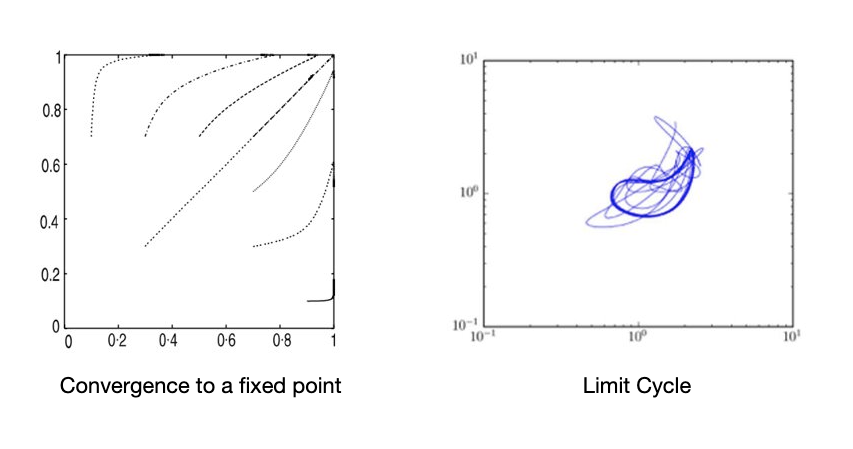
\includegraphics[width=0.5\textwidth]{Figures/DynamicalBehavioursTop.png}
        \end{subfigure}
        
        \begin{subfigure}[b]{0.9 \textwidth}
        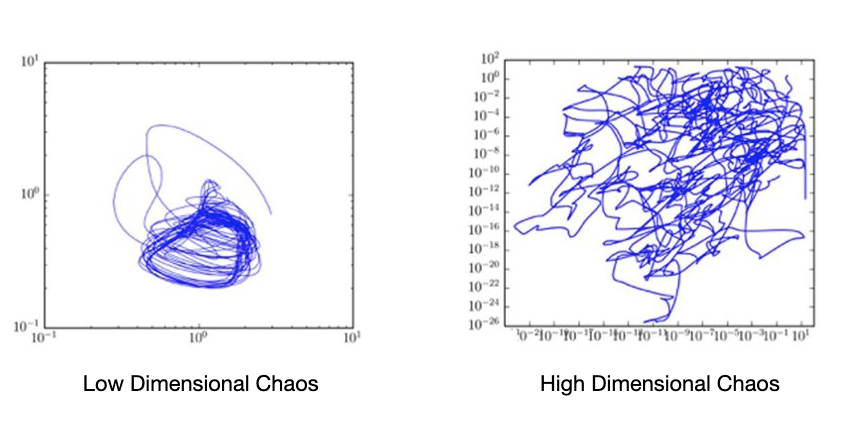
\includegraphics[width=0.5\textwidth]{Figures/DynamicalBehaviourschaos.png}
        \end{subfigure}
        
        \caption{ \label{fig::DynamicalBehaviours} Different types of dynamical behaviour
       displayed
        by learning agents. Here the $x$-axis (resp.~$y$-axis) is the probability with which agent 1 (resp.~agent 2) chooses a given action. a) Figure drawn from \cite{Tuyls2006AnGames}.
        Convergence
        to a unique fixed point in the upper right corner (1, 1). This fixed point is unique, in
        that all trajectories, regardless of initialisation, will converge to this point. b) Limit Cycle, the trajectories converge to cyclic behaviour c,
        d) Chaotic behaviour, here small deviations in the initial conditions can grow
        exponentially. b-d drawn from \cite{Sanders2018}}

    \end{figure}

\subsection{Dynamics of Q-Learning}

The behaviour of a system may be studied given a model of its
dynamics. It is through this process that a wide array of physical
systems, from harmonic pendulums to geophysical fluids, can be
understood. A growing body of research aims to understand
multi-agent reinforcement learning through the lens of its
dynamics. In this light, \cite{Tuyls2006AnGames} presents of derivation of a continuous time dynamical
system describing how agents following a Q-Learning approach adjust the probabilities of choosing actions
as they iteratively play a game. The Q-Learning approach considered requires an agent to choose an action $i$ at step $k+1$ with probability

\begin{equation}
    x_i(k) = \frac{e^{\tau Q_i(k)}}{\sum_j e^{\tau Q_j(k)}}
\end{equation}

where $\tau$ is the \textit{intensity of choice} as defined at the end of this section and $Q_i$ denotes the \textit{Q-value} of an action $i$, which is to be updated at each step according to
%
\begin{equation}
\label{eqn::Qupdate}
    Q_i(k+1) = (1 - \alpha) Q_i(k) + \alpha (r + \gamma \max_j Q_j(k))
\end{equation}

where $\alpha$ is the \textit{step length} parameter defined below, $r$ is the immediate reward received and $\gamma$ is a discount factor.

Through their analysis, Tuyls et al. were able to
arrive at the following dynamical model of Multi-Agent Q-Learning
%
\begin{subequations}
\label{eqn::EOM}
    \begin{equation}
        \frac{\dot{x}_i(t)}{x_i(t)} = \alpha \tau (\sum_{j} a_{ij} y_j - \sum_{i j} x_i a_{ij} y_j)
        + \alpha \sum_j x_j ln(\frac{x_j}{x_i}) 
    \end{equation}
    \begin{equation}
        \frac{\dot{y}_i(t)}{y_i(t)} = \alpha \tau (\sum_{j} b_{ij} x_j - \sum_{i j} y_i b_{ij} x_j)
        + \alpha \sum_j y_j ln(\frac{y_j}{y_i}).
    \end{equation}
\end{subequations}

Here, $\alpha$ and $\tau$ are the parameters of the agent as described at the end of this section. Agent 1 (resp.~agent 2) takes action $i$ with probability
$x_i$ (resp.~$y_j$).
\st{while Agent 2 takes action $j$ with probability $y_j$}. When these actions are taken, the agents
receive payoff $a_{ij}$ and $b_{ji}$ respectively. With these equations, it is possible to
predict the expected behaviour of Q-Learning agentswhich they go on to verify.

It is clear from (\ref{eqn::EOM}) that the long-term strategy selection of
these agents is determined by the parameters $\alpha, \tau$ and the payoffs $a_{ij}, b_{ij}$. In light of this, the following sections aim to address the question presented in the introduction: how do these elements influence the types of behaviours seen during
learning on an iterated game? Specifically, the parameters we will consider are:

\begin{enumerate}
    \item $\alpha \in [0, 1]$: the \textit{step length}. Low values of $\alpha$ denote smaller
    updates. Heuristically, we can consider this to be the memory of the agent: lower $\alpha$
    denotes longer memory.
    \item $\tau \in [0, \infty)$: the \textit{intensity of choice}, as termed by Sanders et al. 
    \cite{Sanders2018}. This is sometimes written as $\beta$ in the literature \cite{Sutton2018}.
    $\tau = 0$ results in all actions being selected with equal probability, regardless of their
    Q-value, whilst $\tau \rightarrow \infty$ results in the action with the highest Q-value chosen
    at every step. This may be considered the \textit{exploration-exploitation parameter}. For greater
    details into these parameters, the interested reader should consult \cite{Sutton2018}.
    \item $\Gamma \in [-1, p-1]$: the \textit{payoff correlation}. Since there are an infinite number of realisations of the payoffs $a_{ij}, b_{ij}$, we instead analyse the behaviour for the average payoff case. To do this, we assume that the payoff matrices are drawn from a multi-variate Gaussian with mean zero and
    covariance matrix parameterised by $\Gamma$. We then average over this Gaussian. $\Gamma = -1$ indicates a zero
    sum game, in which the sum of payoffs for a given action across all agents is 0, resulting in a
    purely competitive game. $\Gamma = p-1$ gives a purely cooperative game in which all agents
    share the same payoffs. The manner in which a game is generated from the choice of $\Gamma$ is
    described in (\ref{eqn::Payoffs}) and follows the same procedure as outlined in \cite{Sanders2018}.
\end{enumerate}

%%%%%%%%%%%%%%%%%%%%%%%%%%%%%%%%%%%%%%%%%%%%%%%%%%%%%%%%%%%%%%%%%%%%%%%%

\section{Stability Analysis of Q-Learning} \label{sec::Theory}

In this section we aim to determine how the choice of parameters $\alpha$ and $\tau$, alongside the choice of payoff matrix, affect the stability of the dynamics of Q-learning. However, as the values in the payoff matrix can take any real number, there are an infinite number of possible realisations of games. Of course, it would not be possible to analyse every possible game, we instead follow the procedure outlined in \cite{Coolen2005} and \cite{Galla2013} to average over these realisations and, instead, analyse the \textit{effective dynamics}, the dynamics averaged over all realisations of payoff matrices. Then, we perform a linear stability analysis around equilibrium points to determine the conditions under which a fixed point is stable.

Our first point of call is to extend the dynamics of Tuyls et al.~in  (\ref{eqn::EOM}a) and (\ref{eqn::EOM}b) \st{and extend it} to a general $p$-player game. This yields the dynamics (\ref{eqn::pEOM}). Here, player $\mu$ chooses action $i_{\mu}$ from its action space $\mathcal{A}$ at time $t$ with probability $\xmu{i}{\mu}$ and receives a reward $\payoff{i}{\mu}$ from its payoff matrix $P^\mu$ depending on its own action and the actions of all other agents $i_{-\mu}$. Formally, the notation $i_{-\mu}$ denotes the set $\{ i_\kappa : \kappa \in \{1, 2, ..., p\} \backslash \{\mu\} \}$ and $-i_{\mu}$ denotes the set $\mathcal{A} \backslash {i_\mu}$.

\begin{equation}
\begin{split}
    \label{eqn::pEOM}
    \frac{\dot{\xmu{i}{\mu}}}{\xmu{i}{\mu}} = \alpha \tau ( \sum_{i_{-\mu}} \payoff{i}{\mu} \prod_{\kappa \neq \mu} \xmu{i}{\kappa} - \\ \sum_{i_\mu i_{-\mu}} \xmu{i}{\mu} \payoff{i}{\mu} \prod_{\kappa \neq \mu} \xmu{i}{\kappa} ) + \alpha \sum_{j_\mu \in -i_\mu} \xmu{j}{\mu} ln \frac{\xmu{j}{\mu}}{\xmu{i}{\mu}}
\end{split}
\end{equation}

We now need to scale the system so that $\sum_{i_\mu} \xmu{i}{\mu} = 1$. The reason for this scaling is that, as the number of agents $p$ and number of actions $N$ increases, the expected payoffs that agent $\xmu{i}{\mu}$ receives becomes less distinguishable across its action space. Therefore, the system must be scaled to ensure appreciable differences across actions, so that the agent can choose its actions appropriately (see the discussion in \cite{Sanders2018} or the Supplementary Material for further details). Accordingly we choose scaled variables (denoted with a tilde) as
%
\begin{eqnarray*}
%    \begin{split}
        \payoff{i}{\mu} & = & \tpayoff{i}{\mu} \sqrt{N^{p-1}}\\
        \xmu{i}{\mu} & = & \frac{\txmu{i}{\mu}}{N} \\
        \talpha & = & \frac{\alpha}{N} \\
        \ttau & = & N^{-(p-1)/2} \tau \\
        \htau & = & N^{-p/2} \tau.
%    \end{split}
\end{eqnarray*}

This yields the scaled equation

\begin{equation}
\begin{split}
    \label{eqn::scaledEOM}
    \frac{\dtxmu{i}{\mu}}{\txmu{i}{\mu}} = \alpha \ttau \left ( \sum_{i_{-\mu}} \tpayoff{i}{\mu} \prod_{\kappa \neq \mu} \txmu{i}{\kappa} \right ) \\ - \alpha \htau \left ( \frac{1}{\sqrt{N}} \sum_{i_\mu i_{-\mu}} \txmu{i}{\mu} \tpayoff{i}{\mu} \prod_{\kappa \neq \mu} \txmu{i}{\kappa} \right ) \\ + \talpha \sum_{j_\mu \in -i_\mu} \txmu{j}{\mu} ln \frac{\txmu{j}{\mu}}{\txmu{i}{\mu}}
\end{split}
\end{equation}

Note that the scaled probabilities now satisfy the constraint $\sum_{i_\mu} \txmu{i}{\mu} = N$. For the remainder of this derivation we concern ourselves only with the scaled system so we drop the tilde notation on $P$ and $x$. 

As mentioned, we now wish to generalise the dynamics to account for all the possible realisations of the payoff matrix. To do this, we assert that the payoff elements (after scaling) are generated by a multivariate Gaussian distribution with mean zero and covariance given as
%
\begin{equation}
\label{eqn::Payoffs}
    \begin{split}
        \mathbb{E}\left [ \payoff{i}{\mu} \payoff{i}{\nu} \right] = \begin{cases}
        \frac{1}{N^{p-1}}  \text{ if } \nu = \mu \\
        \frac{\Gamma}{(p-1) N^{p-1}} \text{ otherwise. }
        \end{cases}
    \end{split}
\end{equation}

The motivation for choosing that the payoffs should be generated by a Gaussian is that it allows for the use of Gaussian identities when determining the average.

\subsection{Generating Functional Analysis}

We then use a generating functional approach as outlined in \cite{Mezard1986} to average the dynamics over this multivariate Gaussian. The generating functional is a method derived from statistical mechanics which allows for expectations to be taken over equations of motion and, more specifically, allows for the analysis of systems with `quenched disorder'. These are variables which are random but held fixed in time as the system evolves (in our case these variables are the payoff elements). The generating functional is given as \cite{SpinGlassTheory}

\begin{equation}
	Z = \int D[\Vec{x}] \prod_i \delta(\textit{equation of motion}_i) exp(i
	\int dt[x_i(t) \psi_i(t)]), 
\end{equation}

where the equations of motion are the Lagrange equations of motion given in (
\ref{eqn::scaledEOM}) and
the fields $\Vec{\psi_i(t)}$ and $\Vec{\phi_i(t)}$ will be set to zero at the end of the
calculation. $\delta$ denotes the Dirac delta function. Implementing our equation of motion yields

\begin{equation}
	\begin{split}
	Z(\Vec{\psi}) = \int D[\Vec{x}, \Vec{\hat{x}}] exp( i \sum_{i, \mu} \int dt [ \hxmu{i} (\frac{\dxmu{i}}{\xmu{i}{\mu}} - \talpha \rho_i^\mu (t) - h_i^\mu (t))]) \times \\ exp(-i \alpha \ttau \sum_{\mu} \sum_{i_\mu, i_{-\mu}} \int dt [\hxmu{i} \payoff{i}{\mu} \prod_{\kappa \neq \mu} \xmu{i}{\kappa} )])) 
    \times \\ exp(-i \alpha \ttau \sum_{\mu} \sum_{j_\mu, i_\mu, i_{-\mu}} \int dt [\hxmu{j}  \xmu{i}{\mu} \payoff{i}{\mu} \prod_{\kappa \neq \mu} \xmu{i}{\kappa}])) 
	\times \\ exp(i \sum_{i, \mu}
	\int dt[\xmu{i} \psi^\mu_i(t)]),
\end{split}
\end{equation}

The last two exponentials contain the payoffs of the game. These are randomly generated using a multivariate gaussian and then held fixed for the rest of the game. As such these comprise the aforementioned 'quenched disorder'. We will average over this quenched disorder (and therefore average over all possible realisations of payoff matrices).

By taking this average, described in further detail in the Supplementary Material, we obtain the \textit{effective dynamics}

\begin{equation}
    \label{eqn::EffectiveDynamics}
    \begin{split}
            \frac{1}{x} \frac{d}{dt} x(t) = \alpha^2 \ttau^2 \Gamma \int dt' \left [G(t, t')C^{p - 2}(t, t') x(t') \right ]\\ + \sqrt{2} \alpha \ttau \eta_1(t) + \sqrt{2} \alpha \htau \eta_0(t) + \talpha \rho(t), 
    \end{split}
\end{equation}

in which we have assumed that all players' actions are independent and drawn from the same initial distribution (\ref{eqn::Payoffs})
and therefore dropped the distinction between players and strategy components. The terms $G, C, \eta_1, \eta_0$ are correlation functions, generated during when averaging the Gaussian. These are given by 

\begin{eqnarray*}
%    \begin{split}
        C(t, t') & = & \mathbb{E}[x(t) x(t')] \\
        \mathbb{E}[\eta_1(t)] & = & 1, \text{ \space } \mathbb{E}[\eta_1(t) \eta_1(t')]  =  C^{p-1}(t, t') \\
        \mathbb{E}[\eta_0(t)] & = & 1, \text{ \space } \mathbb{E}[\eta_0(t) \eta_0(t')] = C^{p}(t, t') \\
        G(t, t') & = & \mathbb{E}\left [ \frac{\delta x(t)}{ \delta \eta_1(t')} \right].
%    \end{split}
\end{eqnarray*}

It is important to note the effect of the former assumption (that all actions of all agents are i.i.d) is substantial. With this assumption, we reduce the second summation term, which couples actions from all agents $\xmu{i}{\mu}$ in (\ref{eqn::EOM}) to the uncoupled term $\sqrt{2} \alpha \htau \eta_0(t)$ in (\ref{eqn::EffectiveDynamics}). This is a strong assumption which is required to analyse the stability of the dynamics in the competitive regime. However, as shown by the experimental evaluation, it does not produce a strong discrepancy in describing the qualitative effect on stability caused by the parameters $\alpha, \Gamma, \tau$.


\subsection{Linear Stability Analysis}

We now analyse the stability of this system in a neighbourhood around the fixed point. This follows a similar procedure as in \cite{Opper1992}, in which the fixed point dynamics are proposed to be perturbed by a disturbance $\xi(t)$ which is drawn from a Gaussian of zero mean and unit variance. The disturbance causes the values of $x(t)$ and $\eta_0(t), \eta_1(t)$ to deviate from their fixed point position $\xfixed, \ezerof, \eonef$ by an amount $\xpert, \ezeropert, \eonepert$.
If we consider only the terms which are linear in these perturbations, we arrive at the dynamics

\begin{equation}
\label{eqn::Linearised}
    \begin{split}
        \frac{d}{dt} \xpert = (\xfixed + \xpert) [ \alpha^2 \ttau^2 \Gamma \xfixed \int dt' [ G(t, t')C^{p - 2}(t, t') ]\\ + \sqrt{2} \alpha \ttau \eonef + \sqrt{2} \alpha \htau \ezerof + \talpha \rho] \\
        + \xfixed [\alpha^2 \ttau^2 \Gamma \int dt' [ G(t, t')C^{p - 2}(t, t') \xpertdash ] \\ + \sqrt{2} \alpha \ttau \eonepert + \sqrt{2} \alpha \htau \ezeropert + \xi(t)].
    \end{split}
\end{equation}

At a fixed point, then, the perturbations $\xpert$ will be zero, leaving

\begin{equation}
    \begin{split}
    \label{eqn::fixed_point}
        0 = \xfixed [ \alpha^2 \ttau^2 \Gamma \xfixed q^{n-1} \chi + \\ + \sqrt{2} \alpha \ttau q^{n/2}z + \sqrt{2} \alpha \htau q^{(n+1)/2} z^{(n+1)/n}],
    \end{split}
\end{equation}

where $\chi = \int dt' G(t - t')$ (at a fixed point where the probabilities do not vary with time, this is equal to $\int dt' G(t, t')$), $\eta_0(t) = q^{n/2}z$ and $z$ is drawn from a Gaussian of zero mean and unit variance and $n = p - 1$. Having arrived at a condition for the fixed point, we then examine the long-term behaviour of the perturbation $\xpert$. To do this, we take the Fourier transform of (\ref{eqn::Linearised}) and analyse its behaviour at $\omega = 0$. After some manipulation, which are given in the Supplementary Material, this gives

\begin{equation}
\begin{split}
        \mathbb{E}[|\mathcal{X}(\omega = 0)|^2] = \frac{1}{\left[ (-\alpha^2 \ttau^2 \Gamma q^{n-1} \chi)^2 - 2 (\alpha \ttau + \alpha \htau)^2 (p-1)q^{p-2}\right]} \\
\end{split}
\end{equation}

As the left hand side of this equation must be greater than zero, we arrive at the condition that, at a fixed point, the long term perturbations must satisfy

\begin{equation}
    \label{eqn::Final}
    0 \leq \left [(\alpha^2 \ttau^2 \Gamma q^{n-1} \chi)^{2} - 2 (\alpha \ttau + \alpha \htau)^2 (p-1)q^{p-2} \right ]
\end{equation}

It should be noted that, to arrive at this result, we have had to take the assumption that $2 >> 1/n$. 


\paragraph{Discussion}
The fixed point condition (\ref{eqn::Final}) yields a number of testable implications, of which we test the validity through in the subsequent section. These implications are as follows.

\begin{enumerate}
    \item Convergence is rare. This is seen by the fact that, for all allowed choices of $\Gamma, \alpha, \tau$, the right hand side of (\ref{eqn::Final}) is positive, which violates the stability criterion. This implies that games, in general, will not converge.
    \item The probability of convergence decreases with increasing $\alpha$, regardless of the choice of $N, p$. We can see this since the right hand side of (\ref{eqn::Final}) tends further away from zero (i.e. further from the region of stability).
    \item At low values of $\alpha$, the game is everywhere convergent, regardless of the choice of $\Gamma$. In fact, the choice of $\Gamma$ does not affect the outcome of the stability analysis at all. This is more easily interpreted from the heatmapts in Figure \ref{fig:theory}.
\end{enumerate}

%%%%%%%%%%%%%%%%%%%%%%%%%%%%%%%%%%%%%%%%%%%%%%%%%%%%%%%%%%%%%%%%%%%%%%%%

\section{Experimental Evaluation} \label{sec:exev}

\begin{figure}
    \centering
    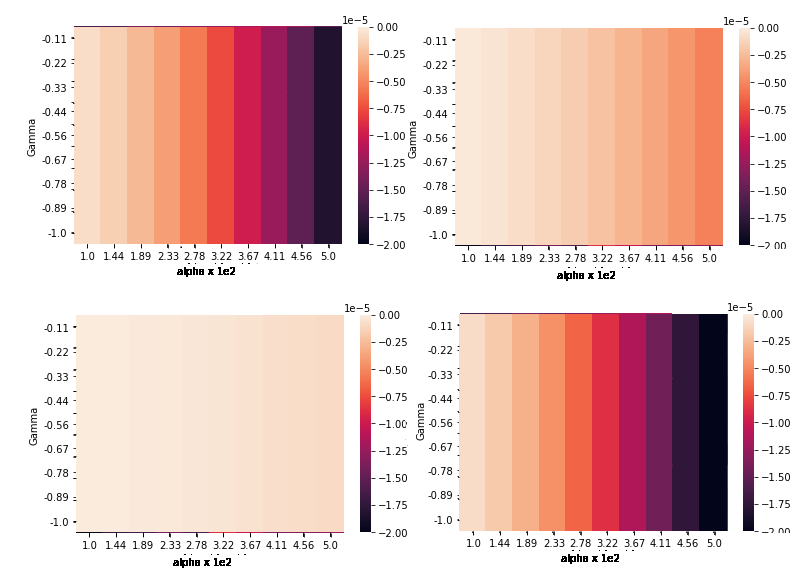
\includegraphics[width = 1.1 \linewidth]{Figures/Theory.png}
    \caption{Results of numerical experiments. The heatmaps show the value of the Liapunov Exponent determined by the procedure outlined in Section~\ref{sec:exev} scaled by $1 \times 10^5$ for convenience. Lighter values show a higher exponent whilst darker values indicate lower values. Each experiment is run with $\tau = 0.05$. (Top Left) $p = 2, N = 2$, (Top Right) $p = 2, N = 4$, (Mid-Left) $p = 2, N = 10$, (Mid-Right) $p = 2, N = 20$, (Bottom) $p = 3, N = 5$.}
    \label{fig:theory}
\end{figure}
%\fb{Can we arrange Fig.~\ref{fig:theory} in a 2x2 square?}

We illustrate these implications in Figure \ref{fig:theory} which plots the value (and takes the absolute value for convenience) obtained by the right hand side of (\ref{eqn::Final}). In order to determine these values, we first had to solve (\ref{eqn::fixed_point}) for \st{the values of} $q$ and $\chi$. We ignore the choice $\xfixed  = 0$, since the proportion of agents who choose a non zero action probability is considered to be 1 \fb{the meaning of this is not clear to me}, an intuitive result \fb{assumption?} which is also considered in \cite{Sanders2018} and \cite{Coolen2005}. As such, we solve for $\xfixed$ using a Newton-Raphson root-finding approach and use the given \fb{obtained} expressions for $q, \chi$ to determine their value \fb{can we give such expressions?}. It should note that this method of finding $\xfixed$ yields only an approximate value and so the $q, \chi$ which are found are estimates of their true value. 

We evaluate (\ref{eqn::Final}) for varying values of $\alpha$ and $\Gamma$, whilst keeping $\tau$ fixed at 0.05 and restricting the range of $\Gamma$ to $[-1, 0]$, as it is only for this range that the solution to (\ref{eqn::fixed_point}) is defined. The range of $\alpha$ is also restricted to $[0.01, 0.05]$ as it is found that for larger values \st{of $\alpha$,} convergence is not seen. 

\fb{Equation} (\ref{eqn::Final}) always evaluates to a positive value, suggesting that Q-learning in games is always unstable. We believe that this is due to the heavy assumptions made during the derivation of the analytic result, the strongest of which was to drop the discrepancy between players and actions, treating each action of each player to be equal \fb{in which sense equal?}. However, even within the error that this assumption generates, it is still clear (and is verified experimentally) that convergence in Q-Learning is rare. We therefore interpret (\ref{eqn::Final}), for given parameters, by determining how close the right hand side is to the stability boundary (i.e., how close the value is to zero). A choice of parameters which evaluates close to the stability boundary has a higher chance of being convergent than one which lies further from the boundary. Therefore, the heat-maps in Figure \ref{fig:theory} should be considered to show the probability of convergence for a choice of $(\alpha, \Gamma)$. Darker regions denote a higher probability of convergence whereas lighter regions are those whose values are further from zero and therefore show a lower probability of convergence.

In addition, we can visualise the implications 2 and 3 in Sec.~\ref{sec::Theory} by comparing the heat-maps. We see in all of the heat-maps that the probability of convergence decreases as $\alpha$ increases (i.e., moving from left to right). At low values of $\alpha$, convergence is seen for all choices of $\Gamma$. However, as $\alpha$ increases, the overall likelihood of convergence rapidly decreases and 
%the convergence 
it is more sensitive to the choice of $\Gamma$. A point to note is the implication that, with the increase of $p$ and $N$ comes a significant increase in the likelihood of convergence. This implication experimental evaluation \fb{?} and therefore can be seen as a limitation of (\ref{eqn::Final}). Instead, it should be viewed that, for a choice of $p, N$, the variation in stability of a system can be determined from $\alpha$ and $\Gamma$.

\subsection{Construction of Numerical Experiments}

To verify \fb{experimentally the theoretical results}, and to examine the underlying structure of stability and chaos in
Multi-Agent Q-Learning, we perform a series of numerical experiments by varying the parameters $\Gamma$ and
$\alpha$ whilst keeping $\tau$ fixed. The purpose 
\st{of this experiment} is to determine a heuristic estimate for the Lyapunov exponent, which measures the degree to which initial conditions which start close to one another converge or diverge as the dynamics evolve \cite{Strogatz2000}. The former indicates a stable system (in the sense of Lyapunov \cite{}) whilst the latter signals instability. The procedure for calculating the Lyapunov exponent is given in (\ref{eq::LiapExpo}).


To generate the numerical simulations in Figure~\ref{fig:NumericalExperiments} we used the
following procedure.
\begin{enumerate}
   \item Fix the paremeters $\tau, \gamma$. The latter is held at 0.5 in all experiments as (\ref{eqn::EOM}) indicates that the value of $\gamma$ does not affect the overall behaviour of the system.
   \item Initialise values of $\Gamma, \alpha$. These will be swept over in the experiment.
\item Generate 5 payoff matrices for both agents by sampling from a multi-variate Gaussian 
(variables are the payoff elements) with mean zero and covariance parameterised by $\Gamma$.
\item Initialise 2 sets of agents (denote their action probabilities as $\Vec{A_1}$ and $\Vec{A_2}$ respectively) each with random initial conditions (i.e., random action probabilities).
\item Allow both sets of agents to learn over a maximum of $1 \times 10^4$ iterations.
\item After 500 iterations measure the distance $\Vec{\delta_1} = |A_2 - A_1|$
\item After 10000 iterations measure the distance $\Vec{\delta_n} = |A_2 - A_1|$
\item Determine \fb{the Lyapunov exponent} 
\begin{eqnarray*}
\label{eq::LiapExpo}
    \lambda_n & = & \max_{i} 10^{-4} ln(\delta_{n, i}/\delta_{1, i})
\end{eqnarray*}
for each action $i$ and average this value over all five realisations of the payoff matrix. 
\end{enumerate}
   
This yields the result shown in Figure~\ref{fig:NumericalExperiments}. We see from this that the stability of the system is highly dependent on
the value of $\alpha$ and (although less so) on $\Gamma$.
   
\begin{figure}[t]
    \centering
    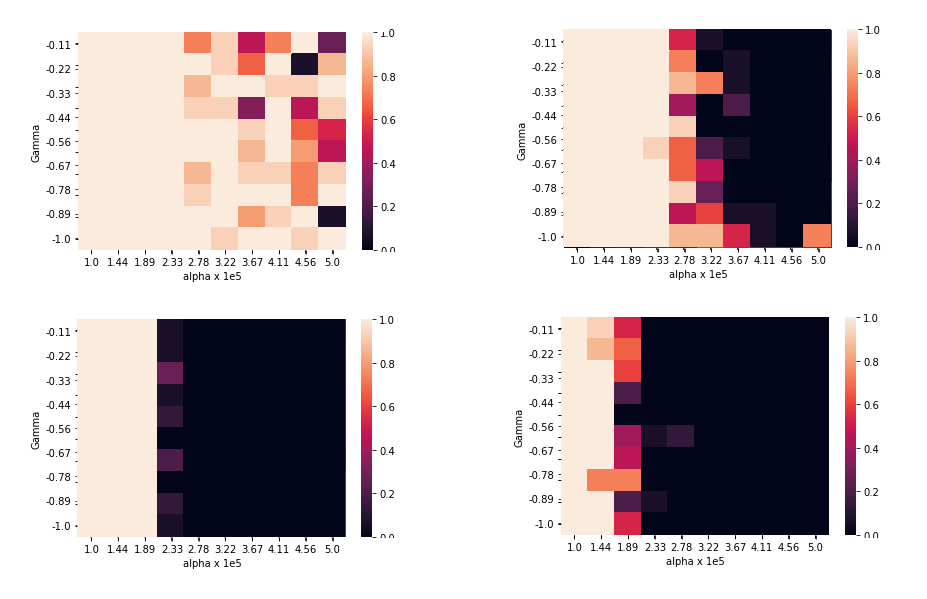
\includegraphics[width = 0.9 \linewidth]{Figures/Experiments.png}
    \caption{Results of numerical experiments. The heat-maps show the value of the Lyapunov Exponent determined by the procedure outlined in this section scaled by $1 \times 10^5$ for convenience. Lighter values show a higher exponent whilst darker values indicate lower values. Each experiment is run with $\tau = 0.05$. (Top Left) $p = 2, N = 2$, (Top Right) $p = 2, N = 4$, (Mid-Left) $p = 2, N = 10$, (Mid-Right) $p = 2, N = 20$, (Bottom) $p = 3, N = 5$.}
    \label{fig:NumericalExperiments}
\end{figure}

\subsection{Discussion}

We note that the numerical experiments confirm the predictions suggested by the analytic results shown in Figure .... We notice that convergence occurs almost only for low values of $\alpha$. This observation remains as we increase the value of $N$. We do, however, notice some discrepancy between the boundary of stability predicted by the analytic result and that revealed in experiments. This is largely due to the assumptions of $N \rightarrow \infty$ and $\frac{1}{p-1} << 2$ made during the derivation. The remaining discrepancy is partially due to the aforementioned error \fb{approximation?} in the calculation of $q$, $\chi$ and \st{partially due to} the fact that the analytic result considers the expected behaviour of Q-Learning. We expect that averaging over a greater number of payoff realisations and initial conditions will yield a more representative assessment of the average behaviour of Q-Learning. However, running these experiments is a computationally expensive procedure: for $p$ players and $N$ actions we require operations on $p$ matrices with $N^{p}$ elements. As such, due to a reduced availability of computational facilities, a large scale averaging was not possible.

A point which we wish to discuss here is the difference in the result found w.r.t.~\cite{Sanders2018}, which considered the stability of \textit{Experience Weighted Attraction} (EWA). \st{and those found in this study.} Namely, Sanders et al.~found that convergence is seen for higher values of $\alpha$, whereas lower values give rise to chaos, the opposite of what is found here. The reason for this can be seen in the update equation of Q-Learning (\ref{eqn::Qupdate}), whereby
\st{in which we see that} 
smaller values of $\alpha$ result in the agent placing a lower weight on the reward received at each step. As such, lower values of $\alpha$ result in the agent taking more conservative steps and yields a higher probability of convergence. In contrast, the update for EWA does not discount the reward received at all and, instead, only discounts the previous knowledge of the Q-value based on higher choices of $\alpha$. In essence, the difference is the fact that Q-Learning discounts new information by a factor of $\alpha$, whilst EWA does not. Yet, the difference in stability caused by this change is significant. We believe this highlights the importance of performing analyses such as the present work; it allows for a method to analytically compare the difference between learning algorithms and, for practitioners, ensure that the appropriate algorithm is chosen for the parameters of their specific task.

A limitation of (\ref{eqn::Final}) is that it predicts that convergence should increase as $N$ and $p$ decreases \fb{or increase?}, a notion that does not seem to hold true in our experimental results. We hypothesize that this is a feature of raising the system to the $N \rightarrow \infty$ limit. \fb{The following paragraph seems a rather daunting criticism of the paper. Any chance it can be rephrased to emphasize the positive contribution?  This assumption means that the analytic result does not lie on the true boundary between convergence and chaos and, in the particular case of Q-Learning, predicts a higher overall probability of convergence than is actually the case.} Instead, as the experiments show, the probability of convergence is higher for games with lower numbers of actions and, in fact, convergence is almost ubiquitous for a 2-player, 2-action game. 

To summarise, we have shown that the analytic result (\ref{eqn::Final}) provides a strong assessment for the effect that $\alpha$, $\Gamma$ and $p$ have on the likelihood of convergence of Q-Learning. We show that the behaviour of the stability line differs from that of EWA and suggest that this shows that a stability analysis is an important mode of analysis for reinforcement learning equations to ensure that parameters are being chosen appropriately to guarantee the safe convergence of learning. 

%%%%%%%%%%%%%%%%%%%%%%%%%%%%%%%%%%%%%%%%%%%%%%%%%%%%%%%%%%%%%%%%%%%%%%%

\section{Conclusion}

In this study, we characterise the behaviours of Q-Learning in $p$-player, $N$-action games. To do this, we analyse the replicator model of Q-Learning derived by Tuyls et al. Specifically, we search for the regions in parameter space where the dynamics are expected to converge to a stable equilibrium and those where learning is unstable. This yields a number of important results. We find that convergence to a unique fixed point is found for low values of $\alpha$, the \textit{step length} of the algorithm and for negatively correlated payoff matrices. As $\alpha$ increases, the likelihood of convergence decreases. For positively correlated payoffs, our analysis no longer guarantees the uniqueness of a fixed point. 


As future work, our first aim is to verify the analytic result at a finer resolution and by averaging over a greater number of payoff realisations. This will give a greater insight into the boundary between convergent and non-convergent behaviour and allow for practitioners to choose their parameters in such a way that convergence to a unique fixed point is expected. In addition we noted that one of the conclusions to our study is that convergence to a unique fixed point is rare in Q-Learning. In fact, complex behaviour (such as the existence of multiple fixed points, limit cycles and chaos) is more likely. We, therefore, aim to characterise these complex behaviours in parameter space both theoretically and numerically.

The present work gives a first step towards considering the stability of Multi-Agent Reinforcement Learning and focuses on the limiting case of stateless normal-form games played by homogeneous agents. As research into the dynamics of Reinforcement Learning algorithms progresses, it would be prudent to apply this analysis to various other algorithm. Algorithms whose dynamics are established, and are therefore open to a stability analysis, include piecewise Q-Learning and Cross Learning. This would provide a strong method by which to compare and provide safety guarantees to different algorithms for a particular use case. 

%%%%%%%%%%%%%%%%%%%%%%%%%%%%%%%%%%%%%%%%%%%%%%%%%%%%%%%%%%%%%%%%%%%%%%%%

%%% The acknowledgments section is defined using the "acks" environment
%%% (rather than an unnumbered section). The use of this environment 
%%% ensures the proper identification of the section in the article 
%%% metadata as well as the consistent spelling of the heading.

\begin{acks}
If you wish to include any acknowledgments in your paper (e.g., to 
people or funding agencies), please do so using the `\texttt{acks}' 
environment. Note that the text of your acknowledgments will be omitted
if you compile your document with the `\texttt{anonymous}' option.
\end{acks}

%%%%%%%%%%%%%%%%%%%%%%%%%%%%%%%%%%%%%%%%%%%%%%%%%%%%%%%%%%%%%%%%%%%%%%%%

%%% The next two lines define, first, the bibliography style to be 
%%% applied, and, second, the bibliography file to be used.

\bibliographystyle{ACM-Reference-Format} 
\bibliography{references}

%%%%%%%%%%%%%%%%%%%%%%%%%%%%%%%%%%%%%%%%%%%%%%%%%%%%%%%%%%%%%%%%%%%%%%%%

\end{document}

%%%%%%%%%%%%%%%%%%%%%%%%%%%%%%%%%%%%%%%%%%%%%%%%%%%%%%%%%%%%%%%%%%%%%%%%


